\documentclass[12pt]{article}
\usepackage{amsmath}
\usepackage{graphicx}
\usepackage{hyperref}
\usepackage[utf8]{inputenc}
\usepackage{geometry}
\usepackage{mathtools}
\usepackage{empheq}
\usepackage{listings}
\usepackage{xcolor}
\usepackage{minted}
\definecolor{LightGray}{gray}{0.9}

\graphicspath{ {./assets/} }
\geometry{margin=0.75in}

\title{CHEN 461 HW 1}
\author{Mark Levchenko}
\date{January 2023}

\begin{document}

\maketitle

\begin{enumerate}
% Problem 2.5
    \item Problem 2.5
    \begin{align*}
        \frac{d M}{d t} &= \rho F_{in} - \rho F_{out} \\
        \frac{d (\rho V)}{d t} &= \rho F_{in} - \rho F_{out} \\
        \intertext{Assume constant density.}
        \rho \frac{d V}{d t} &= \rho F_{in} - \rho F_{out} \\
        \frac{d V}{d t} &= F_{in} - F_{out} \\
        \frac{d (A h)}{d t} &= F_{in} - F_{out} \\
        A \frac{d h}{d t} &= F_{in} - F_{out}
    \end{align*}
    Tank 1:
    \begin{align*}
        A_1 \frac{d h_1}{d t} &= F_{in} - F_{out,1} \\
        F_{out} &\approx c \sqrt{h} \\
        F_{out,1} &= c_1 \sqrt{h_1} \\
        A_1 \frac{d h_1}{d t} &= F_{in} - c_1 \sqrt{h_1} \\
        A_1 &= \pi r_1^2 \\
        \pi r_1^2 \frac{d h_1}{d t} &= F_{in} - c_1 \sqrt{h_1} \\
        \frac{d h_1}{d t} &= \frac{F_{in} - c_1 \sqrt{h_1}}{\pi r_1^2}
    \end{align*}
    Tank 2 is similar except that the outlet of Tank 1 is the inlet of Tank 2:
    \begin{align*}
        \frac{d h_2}{d t} &= \frac{F_{in,2} - c_2 \sqrt{h_2}}{\pi r_2^2} \\
        F_{in,2} = F_{out,1} &= c_1 \sqrt{h_1} \\
        \frac{d h_2}{d t} &= \frac{c_1 \sqrt{h_1} - c_2 \sqrt{h_2}}{\pi r_2^2}
    \end{align*}
    This problem becomes a system of coupled ODEs:
    \begin{empheq}[box=\fbox]{align*}
        \frac{d h_1}{d t} &= \frac{F_{in} - c_1 \sqrt{h_1}}{\pi r_1^2} \\
        \frac{d h_2}{d t} &= \frac{c_1 \sqrt{h_1} - c_2 \sqrt{h_2}}{\pi r_2^2}
    \end{empheq}
    \begin{align*}
        r_1 = r_2 &= 1 \\
        c_1 &= 0.7 \\
        c_2 &= 0.8 \\
        F_{in} &= 1
    \end{align*}
    The system is solved in a computer. The output graph:
    
    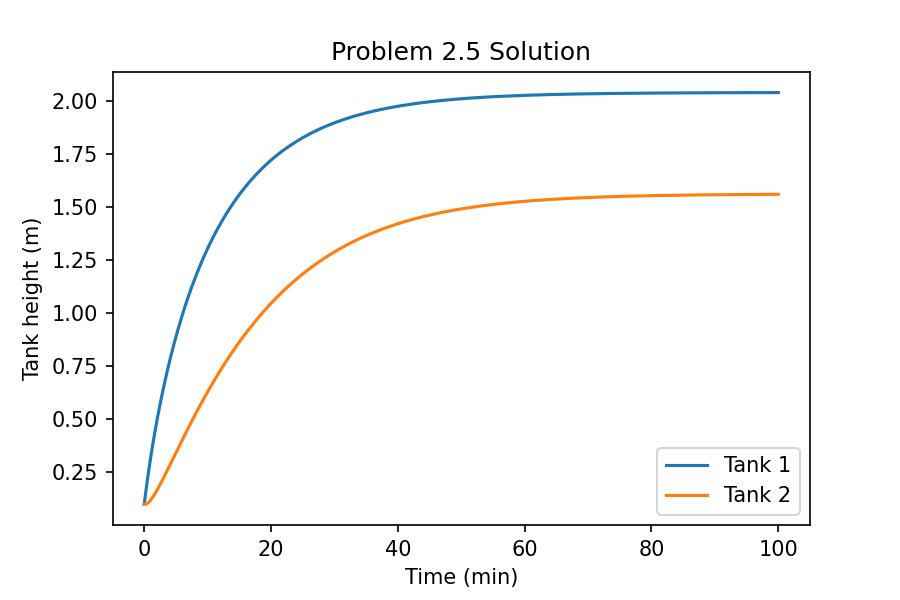
\includegraphics[scale=1]{P_2_5 fig.png}

% Problem 2.6
\newpage
    \item Problem 2.6

    Component R balance at constant volume:
    \begin{align*}
        V \frac{d C_R}{d t} &= F C_{in,R} - F C_R + V \sum^m_{j=1} r_{j,R} \\
        V \frac{d C_R}{d t} &= F C_{in,R} - F C_R - V r_1 + V r_{-1} \\
        r_1 &= k_1 C_R \\
        r_{-1} &= k_{-1} C_P \\
        V \frac{d C_R}{d t} &= F C_{in,R} - F C_R - V k_1 C_R + V k_{-1} C_P \\
        \frac{d C_R}{d t} &= \frac{F}{V} \left( C_{in,R} - C_R \right) - k_1 C_R + k_{-1} C_P
    \end{align*}

    Component P balance:
    \begin{align*}
        V \frac{d C_P}{d t} &= F C_{in,P} - F C_P + V \sum^m_{j=1} r_{j,P} \\
        C_{in,P} &= 0 \\
        V \frac{d C_P}{d t} &= -F C_P + V r_1 - V r_{-1} - V r_2 \\
        r_1 &= k_1 C_R \\
        r_{-1} &= k_{-1} C_P \\
        r_2 &= k_2 C_P^2 \\
        V \frac{d C_P}{d t} &= -F C_P + V k_1 C_R - V k_{-1} C_P - V k_2 C_P^2 \\
        \frac{d C_P}{d t} &= -\frac{F}{V} C_P + k_1 C_R - k_{-1} C_P - k_2 C_P^2
    \end{align*}

    Set of coupled ODEs that define the system:
    \begin{empheq}[box=\fbox]{align*}
        \frac{d C_R}{d t} &= \frac{F}{V} \left( C_{in,R} - C_R \right) - k_1 C_R + k_{-1} C_P \\
        \frac{d C_P}{d t} &= -\frac{F}{V} C_P + k_1 C_R - k_{-1} C_P - k_2 C_P^2
    \end{empheq}

    Input variables: $C_{in,R}$

    State variables: $C_R$, $C_P$

    Output variables: $C_P$

    Parameters: $k_1$, $k_{-1}$, $k_2$, $V$, $F$


% Problem 2.7
\newpage
    \item Problem 2.7

    Overall mass balance:
    \begin{align*}
        \frac{d M}{d t} &= M_{in,1} + M_{in,2} - M_{out} \\
        \rho \frac{d V}{d t} &= \rho F_{in,1} + \rho F_{in,2} - \rho F_{out}
    \end{align*}
    Assume a constant density and that the density of all streams is approximately the same.
    \begin{align*}
        \frac{d V}{d t} &= F_{in,1} + F_{in,2} - F_{out} \\
        V &= Ah \\
        A \frac{d h}{d t} &= F_{in,1} + F_{in,2} - F_{out} \\
        F_{out} &\approx ch \\
        A \frac{d h}{d t} &= F_{in,1} + F_{in,2} - ch
    \end{align*}
    Component mass balance:
    \begin{align*}
        \frac{d (Vw)}{d t} &= w_{in,1} F_{in,1} + w_{in,2} F_{in,2} - w F_{out} \\
        w_{in,1} &= 0 \\
        \frac{d (Vw)}{d t} &= w_{in,2} F_{in,2} - w F_{out} \\
        \frac{d (Vw)}{d t} &= w \frac{d V}{d t} + V \frac{d w}{d t} \\
        w \frac{d V}{d t} + V \frac{d w}{d t} &= w_{in,2} F_{in,2} - w F_{out} \\
        w (F_{in,1} + F_{in,2} - F_{out}) + V \frac{d w}{d t} &= w_{in,2} F_{in,2} - w F_{out} \\
        w F_{in,1} + w F_{in,2} - w F_{out} + V \frac{d w}{d t} &= w_{in,2} F_{in,2} - w F_{out} \\
        V \frac{d w}{d t} &= w_{in,2} F_{in,2} - w (F_{in,1} + F_{in,2}) \\
        A h \frac{d w}{d t} &= w_{in,2} F_{in,2} - w (F_{in,1} + F_{in,2})
    \end{align*}
    Set of coupled ODEs for the mass balance:
    \begin{empheq}[box=\fbox]{align*}
        \frac{d w}{d t} &= \frac{w_{in,2} F_{in,2} - w (F_{in,1} + F_{in,2})}{A h} \\
        \frac{d h}{d t} &= \frac{F_{in,1} + F_{in,2} - ch}{A}
    \end{empheq}
    Energy balance, assuming constant $C_p$ and that $C_v \approx C_p$:
    
    \begin{align*}
        \frac{d (V \rho C_v (T - T_{ref}))}{d t} &= F_{in,1} \rho C_p (T_{in,1} - T_{ref}) + F_{in,2} \rho C_p (T_{in,2} - T_{ref}) - F_{out} \rho C_p (T - T_{ref}) + Q \\
        \intertext{Constant $\rho$ and $C_p$} \\
        \frac{d (V (T - T_{ref}))}{d t} &= F_{in,1} (T_{in,1} - T_{ref}) + F_{in,2} (T_{in,2} - T_{ref}) - F_{out} (T - T_{ref}) + \frac{Q}{\rho C_p} \\
        \frac{d (V (T - T_{ref}))}{d t} &= F_{in,1} T_{in,1} + F_{in,2} T_{in,2} - F_{out} T - T_{ref} ( F_{in,1} + F_{in,2} - F_{out}) + \frac{Q}{\rho C_p} \\
        \frac{d (V (T - T_{ref}))}{d t} &= (T - T_{ref}) \frac{d V}{d t} + V \frac{d (T - T_{ref})}{d t} \\
        \frac{d V}{d t} &= F_{in,1} + F_{in,2} - F_{out} \\
        \frac{d (V (T - T_{ref}))}{d t} &= (T - T_{ref}) (F_{in,1} + F_{in,2} - F_{out}) + V \frac{d (T - T_{ref})}{d t} \\
        \frac{d (V (T - T_{ref}))}{d t} &= T (F_{in,1} + F_{in,2} - F_{out}) - T_{ref} (F_{in,1} + F_{in,2} - F_{out}) + V \frac{d (T - T_{ref})}{d t} \\
        V \frac{d (T - T_{ref})}{d t} &= F_{in,1} T_{in,1} + F_{in,2} T_{in,2} - F_{out} T + \frac{Q}{\rho C_p} - T (F_{in,1} + F_{in,2} - F_{out}) \\
        V \frac{d (T - T_{ref})}{d t} &= F_{in,1} (T_{in,1} - T) + F_{in,2} (T_{in,2} - T) + \frac{Q}{\rho C_p} \\
    \end{align*}
    Final differential equation for energy balance:
    
    \begin{empheq}[box=\fbox]{align*}
        \frac{d T}{d t} &= \frac{F_{in,1} (T_{in,1} - T) + F_{in,2} (T_{in,2} - T) + \frac{Q}{\rho C_p}}{A h}
    \end{empheq}

   Final set of coupled ODEs with mass and energy:

    \begin{empheq}[box=\fbox]{align*}
        \frac{d w}{d t} &= \frac{w_{in,2} F_{in,2} - w (F_{in,1} + F_{in,2})}{A h} \\
        \frac{d h}{d t} &= \frac{F_{in,1} + F_{in,2} - ch}{A} \\
        \frac{d T}{d t} &= \frac{F_{in,1} (T_{in,1} - T) + F_{in,2} (T_{in,2} - T) + \frac{Q}{\rho C_p}}{A h}
    \end{empheq}
\end{enumerate}
\end{document}